\chapter{生成树}

\index{生成树}

图的\key{生成树}包含图的所有节点和图中的一些边，
使得任意两个节点之间都存在路径。
与一般的树一样，生成树是连通的且无环的。
通常有多种方法来构造生成树。

例如，考虑以下图：
\begin{center}
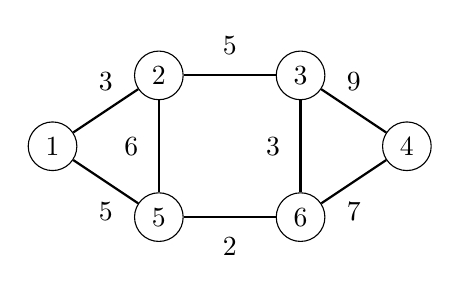
\begin{tikzpicture}[scale=0.9]
\node[draw, circle] (1) at (1.5,2) {$1$};
\node[draw, circle] (2) at (3,3) {$2$};
\node[draw, circle] (3) at (5,3) {$3$};
\node[draw, circle] (4) at (6.5,2) {$4$};
\node[draw, circle] (5) at (3,1) {$5$};
\node[draw, circle] (6) at (5,1) {$6$};
\path[draw,thick,-] (1) -- node[font=\small,label=above:3] {} (2);
\path[draw,thick,-] (2) -- node[font=\small,label=above:5] {} (3);
\path[draw,thick,-] (3) -- node[font=\small,label=above:9] {} (4);
\path[draw,thick,-] (1) -- node[font=\small,label=below:5] {} (5);
\path[draw,thick,-] (5) -- node[font=\small,label=below:2] {} (6);
\path[draw,thick,-] (6) -- node[font=\small,label=below:7] {} (4);
\path[draw,thick,-] (2) -- node[font=\small,label=left:6] {} (5);
\path[draw,thick,-] (3) -- node[font=\small,label=left:3] {} (6);
\end{tikzpicture}
\end{center}
该图的一个生成树如下：
\begin{center}
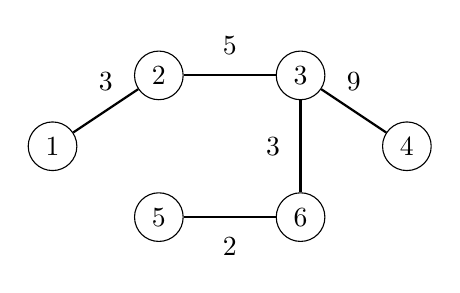
\begin{tikzpicture}[scale=0.9]
\node[draw, circle] (1) at (1.5,2) {$1$};
\node[draw, circle] (2) at (3,3) {$2$};
\node[draw, circle] (3) at (5,3) {$3$};
\node[draw, circle] (4) at (6.5,2) {$4$};
\node[draw, circle] (5) at (3,1) {$5$};
\node[draw, circle] (6) at (5,1) {$6$};
\path[draw,thick,-] (1) -- node[font=\small,label=above:3] {} (2);
\path[draw,thick,-] (2) -- node[font=\small,label=above:5] {} (3);
\path[draw,thick,-] (3) -- node[font=\small,label=above:9] {} (4);
\path[draw,thick,-] (5) -- node[font=\small,label=below:2] {} (6);
\path[draw,thick,-] (3) -- node[font=\small,label=left:3] {} (6);
\end{tikzpicture}
\end{center}

生成树的权重是其所有边的权重之和。
例如，上述生成树的权重为
$3+5+9+3+2=22$。

\index{最小生成树}

\key{最小生成树}
是权重尽可能小的生成树。
示例图的最小生成树权重为20，
可以这样构造：

\begin{center}
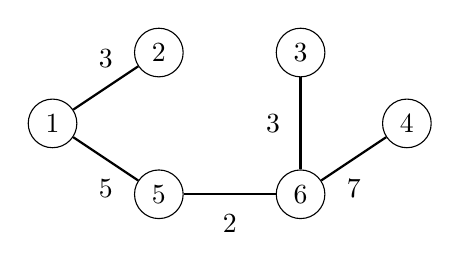
\begin{tikzpicture}[scale=0.9]
\node[draw, circle] (1) at (1.5,2) {$1$};
\node[draw, circle] (2) at (3,3) {$2$};
\node[draw, circle] (3) at (5,3) {$3$};
\node[draw, circle] (4) at (6.5,2) {$4$};
\node[draw, circle] (5) at (3,1) {$5$};
\node[draw, circle] (6) at (5,1) {$6$};

\path[draw,thick,-] (1) -- node[font=\small,label=above:3] {} (2);
\path[draw,thick,-] (1) -- node[font=\small,label=below:5] {} (5);
\path[draw,thick,-] (5) -- node[font=\small,label=below:2] {} (6);
\path[draw,thick,-] (6) -- node[font=\small,label=below:7] {} (4);
\path[draw,thick,-] (3) -- node[font=\small,label=left:3] {} (6);
\end{tikzpicture}
\end{center}

\index{最大生成树}

类似地，\key{最大生成树}
是权重尽可能大的生成树。
示例图的最大生成树权重为32：

\begin{center}
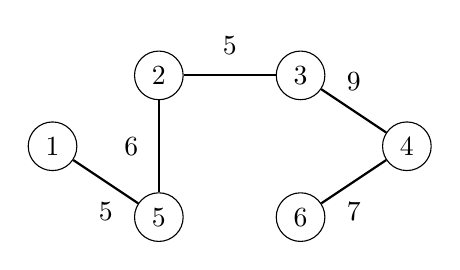
\begin{tikzpicture}[scale=0.9]
\node[draw, circle] (1) at (1.5,2) {$1$};
\node[draw, circle] (2) at (3,3) {$2$};
\node[draw, circle] (3) at (5,3) {$3$};
\node[draw, circle] (4) at (6.5,2) {$4$};
\node[draw, circle] (5) at (3,1) {$5$};
\node[draw, circle] (6) at (5,1) {$6$};
\path[draw,thick,-] (2) -- node[font=\small,label=above:5] {} (3);
\path[draw,thick,-] (3) -- node[font=\small,label=above:9] {} (4);
\path[draw,thick,-] (1) -- node[font=\small,label=below:5] {} (5);
\path[draw,thick,-] (6) -- node[font=\small,label=below:7] {} (4);
\path[draw,thick,-] (2) -- node[font=\small,label=left:6] {} (5);
\end{tikzpicture}
\end{center}

注意，一个图可能有多个
最小生成树和最大生成树，
因此它们不是唯一的。

事实证明，有几种贪心方法
可以用来构造最小生成树和最大生成树。
在本章中，我们讨论两种算法，
它们按照权重的顺序处理图的边。
我们重点讨论最小生成树的求解，
但同样的算法可以通过按相反顺序处理边来
找到最大生成树。

\section{Kruskal算法}

\index{Kruskal算法}

在\key{Kruskal算法}\footnote{该算法于1956年由J. B. Kruskal发表\cite{kru56}。}中，初始生成树
只包含图的节点，不包含任何边。
然后算法按照权重的顺序遍历边，
如果添加某条边不会形成环，
则将该边添加到树中。

该算法维护树的连通分量。
初始时，图中的每个节点
属于一个单独的连通分量。
每当一条边被添加到树中时，
两个连通分量就被合并。
最终，所有节点属于同一个连通分量，
最小生成树就找到了。

\subsubsection{示例}

\begin{samepage}
让我们来看看Kruskal算法如何处理
以下图：
\begin{center}
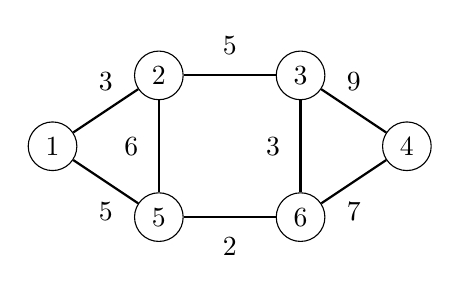
\begin{tikzpicture}[scale=0.9]
\node[draw, circle] (1) at (1.5,2) {$1$};
\node[draw, circle] (2) at (3,3) {$2$};
\node[draw, circle] (3) at (5,3) {$3$};
\node[draw, circle] (4) at (6.5,2) {$4$};
\node[draw, circle] (5) at (3,1) {$5$};
\node[draw, circle] (6) at (5,1) {$6$};
\path[draw,thick,-] (1) -- node[font=\small,label=above:3] {} (2);
\path[draw,thick,-] (2) -- node[font=\small,label=above:5] {} (3);
\path[draw,thick,-] (3) -- node[font=\small,label=above:9] {} (4);
\path[draw,thick,-] (1) -- node[font=\small,label=below:5] {} (5);
\path[draw,thick,-] (5) -- node[font=\small,label=below:2] {} (6);
\path[draw,thick,-] (6) -- node[font=\small,label=below:7] {} (4);
\path[draw,thick,-] (2) -- node[font=\small,label=left:6] {} (5);
\path[draw,thick,-] (3) -- node[font=\small,label=left:3] {} (6);
\end{tikzpicture}
\end{center}
\end{samepage}

\begin{samepage}
算法的第一步是将边按权重的递增顺序排序。
结果如下表：

\begin{tabular}{ll}
\\
边 & 权重 \\
\hline
5--6 & 2 \\
1--2 & 3 \\
3--6 & 3 \\
1--5 & 5 \\
2--3 & 5 \\
2--5 & 6 \\
4--6 & 7 \\
3--4 & 9 \\
\\
\end{tabular}
\end{samepage}

之后，算法遍历列表，
如果边连接了两个不同的连通分量，
就将该边添加到树中。

初始时，每个节点在自己的连通分量中：

\begin{center}
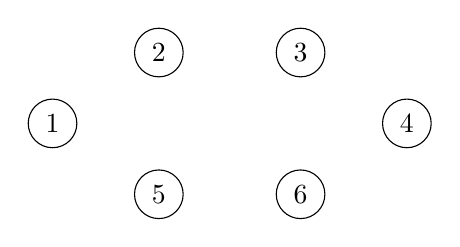
\begin{tikzpicture}[scale=0.9]
\node[draw, circle] (1) at (1.5,2) {$1$};
\node[draw, circle] (2) at (3,3) {$2$};
\node[draw, circle] (3) at (5,3) {$3$};
\node[draw, circle] (4) at (6.5,2) {$4$};
\node[draw, circle] (5) at (3,1) {$5$};
\node[draw, circle] (6) at (5,1) {$6$};
%\path[draw,thick,-] (1) -- node[font=\small,label=above:3] {} (2);
%\path[draw,thick,-] (2) -- node[font=\small,label=above:5] {} (3);
%\path[draw,thick,-] (3) -- node[font=\small,label=above:9] {} (4);
%\path[draw,thick,-] (1) -- node[font=\small,label=below:5] {} (5);
%\path[draw,thick,-] (5) -- node[font=\small,label=below:2] {} (6);
%\path[draw,thick,-] (6) -- node[font=\small,label=below:7] {} (4);
%\path[draw,thick,-] (2) -- node[font=\small,label=left:6] {} (5);
%\path[draw,thick,-] (3) -- node[font=\small,label=left:3] {} (6);
\end{tikzpicture}
\end{center}
第一个被添加到树中的边
是边5--6，它通过合并连通分量$\{5\}$和$\{6\}$
创建了连通分量$\{5,6\}$：

\begin{center}
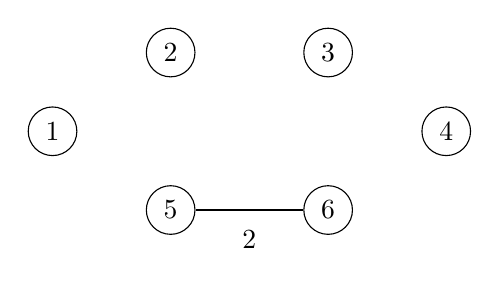
\begin{tikzpicture}
\node[draw, circle] (1) at (1.5,2) {$1$};
\node[draw, circle] (2) at (3,3) {$2$};
\node[draw, circle] (3) at (5,3) {$3$};
\node[draw, circle] (4) at (6.5,2) {$4$};
\node[draw, circle] (5) at (3,1) {$5$};
\node[draw, circle] (6) at (5,1) {$6$};

%\path[draw,thick,-] (1) -- node[font=\small,label=above:3] {} (2);
%\path[draw,thick,-] (2) -- node[font=\small,label=above:5] {} (3);
%\path[draw,thick,-] (3) -- node[font=\small,label=above:9] {} (4);
%\path[draw,thick,-] (1) -- node[font=\small,label=below:5] {} (5);
\path[draw,thick,-] (5) -- node[font=\small,label=below:2] {} (6);
%\path[draw,thick,-] (6) -- node[font=\small,label=below:7] {} (4);
%\path[draw,thick,-] (2) -- node[font=\small,label=left:6] {} (5);
%\path[draw,thick,-] (3) -- node[font=\small,label=left:3] {} (6);
\end{tikzpicture}
\end{center}
之后，边1--2、3--6和1--5以类似的方式被添加：

\begin{center}
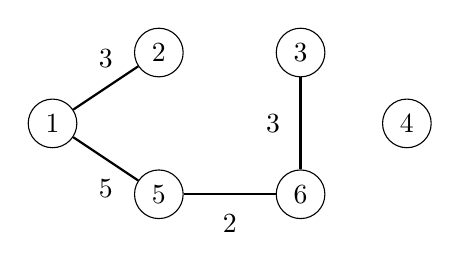
\begin{tikzpicture}[scale=0.9]
\node[draw, circle] (1) at (1.5,2) {$1$};
\node[draw, circle] (2) at (3,3) {$2$};
\node[draw, circle] (3) at (5,3) {$3$};
\node[draw, circle] (4) at (6.5,2) {$4$};
\node[draw, circle] (5) at (3,1) {$5$};
\node[draw, circle] (6) at (5,1) {$6$};

\path[draw,thick,-] (1) -- node[font=\small,label=above:3] {} (2);
%\path[draw,thick,-] (2) -- node[font=\small,label=above:5] {} (3);
%\path[draw,thick,-] (3) -- node[font=\small,label=above:9] {} (4);
\path[draw,thick,-] (1) -- node[font=\small,label=below:5] {} (5);
\path[draw,thick,-] (5) -- node[font=\small,label=below:2] {} (6);
%\path[draw,thick,-] (6) -- node[font=\small,label=below:7] {} (4);
%\path[draw,thick,-] (2) -- node[font=\small,label=left:6] {} (5);
\path[draw,thick,-] (3) -- node[font=\small,label=left:3] {} (6);
\end{tikzpicture}
\end{center}

在这些步骤之后，大多数连通分量已被合并，
树中有两个连通分量：
$\{1,2,3,5,6\}$和$\{4\}$。

列表中的下一条边是2--3，
但它不会被包含在树中，因为
节点2和3已经在同一个连通分量中了。
同理，边2--5也不会被包含在树中。

\begin{samepage}
最后，边4--6将被包含在树中：

\begin{center}
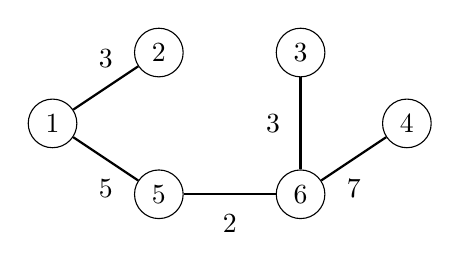
\begin{tikzpicture}[scale=0.9]
\node[draw, circle] (1) at (1.5,2) {$1$};
\node[draw, circle] (2) at (3,3) {$2$};
\node[draw, circle] (3) at (5,3) {$3$};
\node[draw, circle] (4) at (6.5,2) {$4$};
\node[draw, circle] (5) at (3,1) {$5$};
\node[draw, circle] (6) at (5,1) {$6$};

\path[draw,thick,-] (1) -- node[font=\small,label=above:3] {} (2);
%\path[draw,thick,-] (2) -- node[font=\small,label=above:5] {} (3);
%\path[draw,thick,-] (3) -- node[font=\small,label=above:9] {} (4);
\path[draw,thick,-] (1) -- node[font=\small,label=below:5] {} (5);
\path[draw,thick,-] (5) -- node[font=\small,label=below:2] {} (6);
\path[draw,thick,-] (6) -- node[font=\small,label=below:7] {} (4);
%\path[draw,thick,-] (2) -- node[font=\small,label=left:6] {} (5);
\path[draw,thick,-] (3) -- node[font=\small,label=left:3] {} (6);
\end{tikzpicture}
\end{center}
\end{samepage}

此后，算法不会再添加任何
新边，因为图已经连通，
任意两个节点之间都存在路径。
最终的图是一棵最小生成树，
其权重为$2+3+3+5+7=20$。

\subsubsection{为什么这有效？}

Kruskal算法为什么有效是一个好问题。
为什么贪心策略能保证我们找到
最小生成树？

让我们看看如果图中权重最小的边
\emph{不}被包含在生成树中会发生什么。
例如，假设前述图的一个生成树
不包含权重最小的边5--6。
我们不知道这样一棵生成树的确切结构，
但无论如何它必须包含一些边。
假设这棵树如下：

\begin{center}
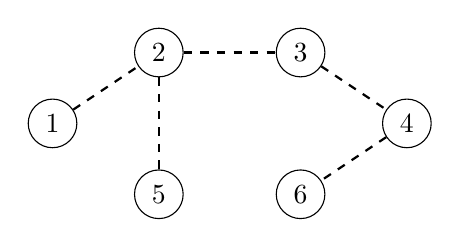
\begin{tikzpicture}[scale=0.9]
\node[draw, circle] (1) at (1.5,2) {$1$};
\node[draw, circle] (2) at (3,3) {$2$};
\node[draw, circle] (3) at (5,3) {$3$};
\node[draw, circle] (4) at (6.5,2) {$4$};
\node[draw, circle] (5) at (3,1) {$5$};
\node[draw, circle] (6) at (5,1) {$6$};

\path[draw,thick,-,dashed] (1) -- (2);
\path[draw,thick,-,dashed] (2) -- (5);
\path[draw,thick,-,dashed] (2) -- (3);
\path[draw,thick,-,dashed] (3) -- (4);
\path[draw,thick,-,dashed] (4) -- (6);
\end{tikzpicture}
\end{center}

然而，上述树不可能
是该图的最小生成树。
原因是我们可以从树中移除一条边，
并用权重最小的边5--6替换它。
这会生成一棵权重\emph{更小}的生成树：

\begin{center}
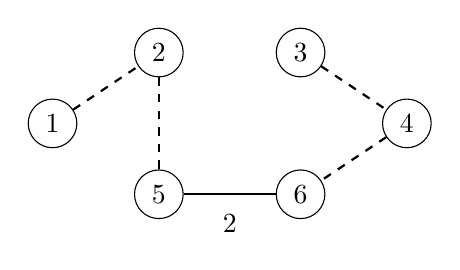
\begin{tikzpicture}[scale=0.9]
\node[draw, circle] (1) at (1.5,2) {$1$};
\node[draw, circle] (2) at (3,3) {$2$};
\node[draw, circle] (3) at (5,3) {$3$};
\node[draw, circle] (4) at (6.5,2) {$4$};
\node[draw, circle] (5) at (3,1) {$5$};
\node[draw, circle] (6) at (5,1) {$6$};

\path[draw,thick,-,dashed] (1) -- (2);
\path[draw,thick,-,dashed] (2) -- (5);
\path[draw,thick,-,dashed] (3) -- (4);
\path[draw,thick,-,dashed] (4) -- (6);
\path[draw,thick,-] (5) -- node[font=\small,label=below:2] {} (6);
\end{tikzpicture}
\end{center}

因此，将权重最小的边
包含在树中以生成最小生成树
总是最优的。
使用类似的论证，我们可以证明按权重顺序
添加下一条边到树中也是最优的，
以此类推。
因此，Kruskal算法能正确工作并
总是产生最小生成树。

\subsubsection{实现}

在实现Kruskal算法时，
使用图的边表表示
非常方便。
算法的第一阶段以$O(m \log m)$的时间
对列表中的边进行排序。
之后，算法的第二阶段
按如下方式构建最小生成树：

\begin{lstlisting}
for (...) {
  if (!same(a,b)) unite(a,b);
}
\end{lstlisting}

循环遍历列表中的边，
每次处理一条边$a$--$b$，
其中$a$和$b$是两个节点。
需要两个函数：
函数\texttt{same}判断$a$和$b$
是否在同一个连通分量中，
函数\texttt{unite}合并
包含$a$和$b$的连通分量。

问题在于如何高效地实现
函数\texttt{same}和\texttt{unite}。
一种可能的实现方式是将
函数\texttt{same}实现为图遍历，
检查是否可以从节点$a$到达节点$b$。
然而，这样一个函数的时间复杂度
为$O(n+m)$，
由此得到的算法会很慢，
因为函数\texttt{same}需要对图中的每条边都调用一次。

我们将使用并查集结构来解决这个问题，
它能在$O(\log n)$时间内实现这两个函数。
因此，Kruskal算法的时间复杂度
（在对边表排序之后）
为$O(m \log n)$。

\section{并查集结构}

\index{并查集结构}

\key{并查集结构}维护
一个集合的集合。
这些集合是互不相交的，因此没有元素
属于多个集合。
支持两个$O(\log n)$时间的操作：
\texttt{unite}操作合并两个集合，
\texttt{find}操作查找包含给定元素的集合的代表元素\footnote{这里介绍的结构
于1971年由J. D. Hopcroft和J. D. Ullman提出\cite{hop71}。
后来，在1975年，R. E. Tarjan研究了一种更复杂的变体\cite{tar75}，
该变体如今在许多算法教科书中都有讨论。}。

\subsubsection{结构}

在并查集结构中，每个集合中的一个元素
是该集合的代表元素，
从集合中任何其他元素到代表元素
都有一条链。
例如，假设集合为
$\{1,4,7\}$、$\{5\}$和$\{2,3,6,8\}$：
\begin{center}
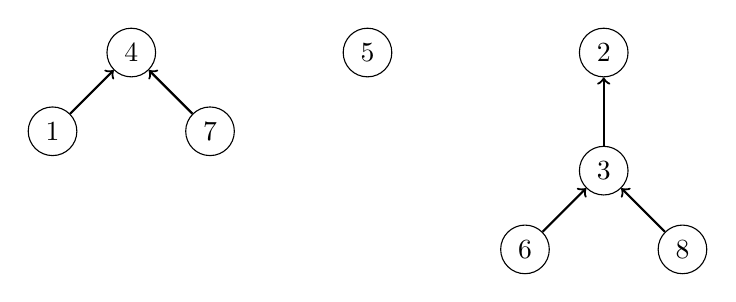
\begin{tikzpicture}
\node[draw, circle] (1) at (0,-1) {$1$};
\node[draw, circle] (2) at (7,0) {$2$};
\node[draw, circle] (3) at (7,-1.5) {$3$};
\node[draw, circle] (4) at (1,0) {$4$};
\node[draw, circle] (5) at (4,0) {$5$};
\node[draw, circle] (6) at (6,-2.5) {$6$};
\node[draw, circle] (7) at (2,-1) {$7$};
\node[draw, circle] (8) at (8,-2.5) {$8$};

\path[draw,thick,->] (1) -- (4);
\path[draw,thick,->] (7) -- (4);

\path[draw,thick,->] (3) -- (2);
\path[draw,thick,->] (6) -- (3);
\path[draw,thick,->] (8) -- (3);

\end{tikzpicture}
\end{center}
在这种情况下，各集合的代表元素
分别为4、5和2。
我们可以通过沿着从该元素开始的链
来找到任何元素的代表元素。
例如，元素2是
元素6的代表元素，因为
我们沿着链$6 \rightarrow 3 \rightarrow 2$行进。
两个元素属于同一个集合
当且仅当它们的代表元素相同。

两个集合可以通过将一个集合的代表元素
连接到另一个集合的代表元素来合并。
例如，集合
$\{1,4,7\}$和$\{2,3,6,8\}$
可以按如下方式合并：
\begin{center}
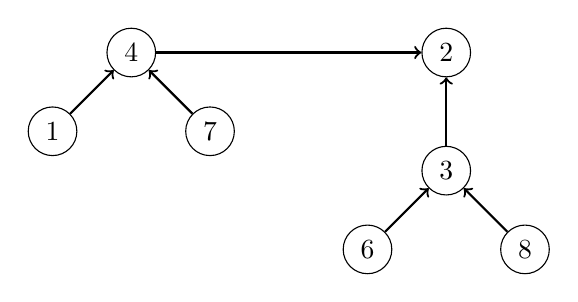
\begin{tikzpicture}
\node[draw, circle] (1) at (2,-1) {$1$};
\node[draw, circle] (2) at (7,0) {$2$};
\node[draw, circle] (3) at (7,-1.5) {$3$};
\node[draw, circle] (4) at (3,0) {$4$};
\node[draw, circle] (6) at (6,-2.5) {$6$};
\node[draw, circle] (7) at (4,-1) {$7$};
\node[draw, circle] (8) at (8,-2.5) {$8$};

\path[draw,thick,->] (1) -- (4);
\path[draw,thick,->] (7) -- (4);

\path[draw,thick,->] (3) -- (2);
\path[draw,thick,->] (6) -- (3);
\path[draw,thick,->] (8) -- (3);

\path[draw,thick,->] (4) -- (2);
\end{tikzpicture}
\end{center}

得到的集合包含元素
$\{1,2,3,4,6,7,8\}$。
从此，元素2成为整个集合的代表元素，
而旧代表元素4指向元素2。

并查集结构的效率取决于
集合如何合并。
事实证明，我们可以遵循一个简单的策略：
始终将\emph{较小}集合的代表元素
连接到\emph{较大}集合的代表元素
（或者如果两个集合大小相同，
可以任意选择）。
使用这种策略，任何链的长度
都是$O(\log n)$，因此我们可以
通过沿着相应的链高效地找到任何元素的代表元素。

\subsubsection{实现}

并查集结构可以使用数组来实现。
在以下实现中，
数组\texttt{link}为每个元素存储
链中的下一个元素，
如果该元素是代表元素则存储其自身，
数组\texttt{size}为每个代表元素
指示相应集合的大小。

初始时，每个元素属于一个单独的集合：
\begin{lstlisting}
for (int i = 1; i <= n; i++) link[i] = i;
for (int i = 1; i <= n; i++) size[i] = 1;
\end{lstlisting}

函数\texttt{find}返回元素$x$的代表元素。
可以通过沿着从$x$开始的链
来找到代表元素。

\begin{lstlisting}
int find(int x) {
    while (x != link[x]) x = link[x];
    return x;
}
\end{lstlisting}

函数\texttt{same}检查
元素$a$和$b$是否属于同一个集合。
这可以通过使用
函数\texttt{find}轻松完成：

\begin{lstlisting}
bool same(int a, int b) {
    return find(a) == find(b);
}
\end{lstlisting}

\begin{samepage}
函数\texttt{unite}合并
包含元素$a$和$b$的集合
（这两个元素必须在不同的集合中）。
该函数首先找到各集合的代表元素，
然后将较小的集合连接到较大的集合。

\begin{lstlisting}
void unite(int a, int b) {
    a = find(a);
    b = find(b);
    if (size[a] < size[b]) swap(a,b);
    size[a] += size[b];
    link[b] = a;
}
\end{lstlisting}
\end{samepage}

函数\texttt{find}的时间复杂度
为$O(\log n)$，前提是每条链的长度为$O(\log n)$。
在这种情况下，函数\texttt{same}和\texttt{unite}
也在$O(\log n)$时间内完成。
函数\texttt{unite}通过将
较小的集合连接到较大的集合来确保
每条链的长度为$O(\log n)$。

\section{Prim算法}

\index{Prim算法}

\key{Prim算法}\footnote{该算法以R. C. Prim的名字命名，
他于1957年发表了该算法\cite{pri57}。
然而，同样的算法早在1930年
就已由V. Jarník发现。}是另一种
寻找最小生成树的方法。
该算法首先将一个任意节点
添加到树中。
之后，算法总是选择一条
权重最小的边来将一个新节点添加到树中。
最终，所有节点都被添加到树中，
最小生成树就找到了。

Prim算法类似于Dijkstra算法。
区别在于Dijkstra算法总是选择
距离起始节点最近的边，
而Prim算法只是简单地将
权重最小且能将新节点添加到树中的边选入。

\subsubsection{示例}

让我们来看看Prim算法在
以下图中是如何工作的：

\begin{center}
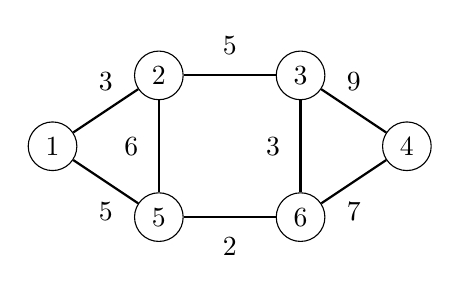
\begin{tikzpicture}[scale=0.9]
\node[draw, circle] (1) at (1.5,2) {$1$};
\node[draw, circle] (2) at (3,3) {$2$};
\node[draw, circle] (3) at (5,3) {$3$};
\node[draw, circle] (4) at (6.5,2) {$4$};
\node[draw, circle] (5) at (3,1) {$5$};
\node[draw, circle] (6) at (5,1) {$6$};
\path[draw,thick,-] (1) -- node[font=\small,label=above:3] {} (2);
\path[draw,thick,-] (2) -- node[font=\small,label=above:5] {} (3);
\path[draw,thick,-] (3) -- node[font=\small,label=above:9] {} (4);
\path[draw,thick,-] (1) -- node[font=\small,label=below:5] {} (5);
\path[draw,thick,-] (5) -- node[font=\small,label=below:2] {} (6);
\path[draw,thick,-] (6) -- node[font=\small,label=below:7] {} (4);
\path[draw,thick,-] (2) -- node[font=\small,label=left:6] {} (5);
\path[draw,thick,-] (3) -- node[font=\small,label=left:3] {} (6);

%\path[draw=red,thick,-,line width=2pt] (5) -- (6);
\end{tikzpicture}
\end{center}
初始时，节点之间没有边：
\begin{center}
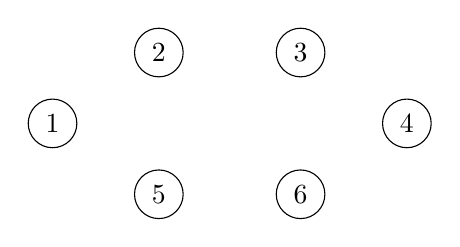
\begin{tikzpicture}[scale=0.9]
\node[draw, circle] (1) at (1.5,2) {$1$};
\node[draw, circle] (2) at (3,3) {$2$};
\node[draw, circle] (3) at (5,3) {$3$};
\node[draw, circle] (4) at (6.5,2) {$4$};
\node[draw, circle] (5) at (3,1) {$5$};
\node[draw, circle] (6) at (5,1) {$6$};
%\path[draw,thick,-] (1) -- node[font=\small,label=above:3] {} (2);
%\path[draw,thick,-] (2) -- node[font=\small,label=above:5] {} (3);
%\path[draw,thick,-] (3) -- node[font=\small,label=above:9] {} (4);
%\path[draw,thick,-] (1) -- node[font=\small,label=below:5] {} (5);
%\path[draw,thick,-] (5) -- node[font=\small,label=below:2] {} (6);
%\path[draw,thick,-] (6) -- node[font=\small,label=below:7] {} (4);
%\path[draw,thick,-] (2) -- node[font=\small,label=left:6] {} (5);
%\path[draw,thick,-] (3) -- node[font=\small,label=left:3] {} (6);
\end{tikzpicture}
\end{center}
任意节点都可以作为起始节点，
所以我们选择节点1。
首先，我们通过权重为3的边
添加节点2：
\begin{center}
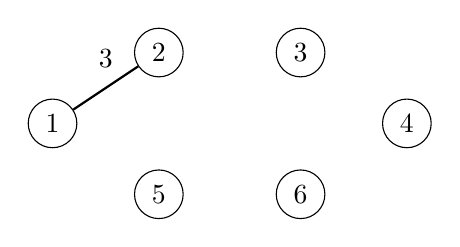
\begin{tikzpicture}[scale=0.9]
\node[draw, circle] (1) at (1.5,2) {$1$};
\node[draw, circle] (2) at (3,3) {$2$};
\node[draw, circle] (3) at (5,3) {$3$};
\node[draw, circle] (4) at (6.5,2) {$4$};
\node[draw, circle] (5) at (3,1) {$5$};
\node[draw, circle] (6) at (5,1) {$6$};
\path[draw,thick,-] (1) -- node[font=\small,label=above:3] {} (2);
%\path[draw,thick,-] (2) -- node[font=\small,label=above:5] {} (3);
%\path[draw,thick,-] (3) -- node[font=\small,label=above:9] {} (4);
%\path[draw,thick,-] (1) -- node[font=\small,label=below:5] {} (5);
%\path[draw,thick,-] (5) -- node[font=\small,label=below:2] {} (6);
%\path[draw,thick,-] (6) -- node[font=\small,label=below:7] {} (4);
%\path[draw,thick,-] (2) -- node[font=\small,label=left:6] {} (5);
%\path[draw,thick,-] (3) -- node[font=\small,label=left:3] {} (6);
\end{tikzpicture}
\end{center}

之后，有两条权重为5的边，
所以我们可以将节点3或节点5添加到树中。
让我们先添加节点3：
\begin{center}
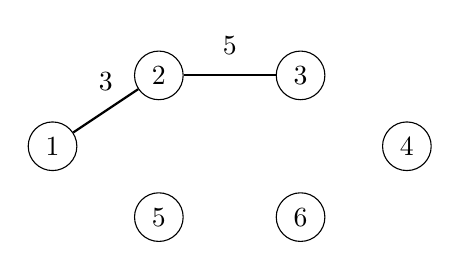
\begin{tikzpicture}[scale=0.9]
\node[draw, circle] (1) at (1.5,2) {$1$};
\node[draw, circle] (2) at (3,3) {$2$};
\node[draw, circle] (3) at (5,3) {$3$};
\node[draw, circle] (4) at (6.5,2) {$4$};
\node[draw, circle] (5) at (3,1) {$5$};
\node[draw, circle] (6) at (5,1) {$6$};
\path[draw,thick,-] (1) -- node[font=\small,label=above:3] {} (2);
\path[draw,thick,-] (2) -- node[font=\small,label=above:5] {} (3);
%\path[draw,thick,-] (3) -- node[font=\small,label=above:9] {} (4);
%\path[draw,thick,-] (1) -- node[font=\small,label=below:5] {} (5);
%\path[draw,thick,-] (5) -- node[font=\small,label=below:2] {} (6);
%\path[draw,thick,-] (6) -- node[font=\small,label=below:7] {} (4);
%\path[draw,thick,-] (2) -- node[font=\small,label=left:6] {} (5);
%\path[draw,thick,-] (3) -- node[font=\small,label=left:3] {} (6);
\end{tikzpicture}
\end{center}

\begin{samepage}
该过程继续进行，直到所有节点都被包含在树中：
\begin{center}
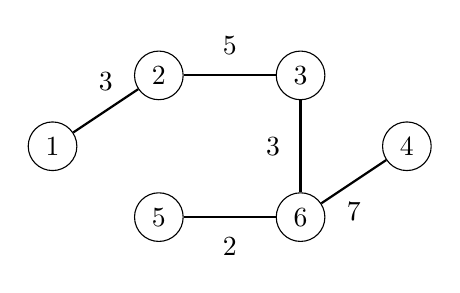
\begin{tikzpicture}[scale=0.9]
\node[draw, circle] (1) at (1.5,2) {$1$};
\node[draw, circle] (2) at (3,3) {$2$};
\node[draw, circle] (3) at (5,3) {$3$};
\node[draw, circle] (4) at (6.5,2) {$4$};
\node[draw, circle] (5) at (3,1) {$5$};
\node[draw, circle] (6) at (5,1) {$6$};
\path[draw,thick,-] (1) -- node[font=\small,label=above:3] {} (2);
\path[draw,thick,-] (2) -- node[font=\small,label=above:5] {} (3);
%\path[draw,thick,-] (3) -- node[font=\small,label=above:9] {} (4);
%\path[draw,thick,-] (1) -- node[font=\small,label=below:5] {} (5);
\path[draw,thick,-] (5) -- node[font=\small,label=below:2] {} (6);
\path[draw,thick,-] (6) -- node[font=\small,label=below:7] {} (4);
%\path[draw,thick,-] (2) -- node[font=\small,label=left:6] {} (5);
\path[draw,thick,-] (3) -- node[font=\small,label=left:3] {} (6);
\end{tikzpicture}
\end{center}
\end{samepage}

\subsubsection{实现}

与Dijkstra算法一样，Prim算法可以
使用优先队列来高效实现。
优先队列应包含所有可以通过单条边连接到
当前连通分量的节点，
按对应边的权重递增排列。

Prim算法的时间复杂度为
$O(n + m \log m)$，与Dijkstra算法的
时间复杂度相同。
在实际应用中，Prim算法和Kruskal算法
都是高效的，选择哪种算法
取决于个人喜好。
不过，大多数竞赛选手使用Kruskal算法。